\newpage

\section{État de l'art}
\subsection{Méthodes de projection de liquides}
\subsubsection{Bombe spray}
Pour constituer des écrans de turbulence aisément, l'approche de la bombe de spray pour les cheveux
, ou de laque transparente pour surfaces a été employée.
\begin{figure}[H]
    \centering
    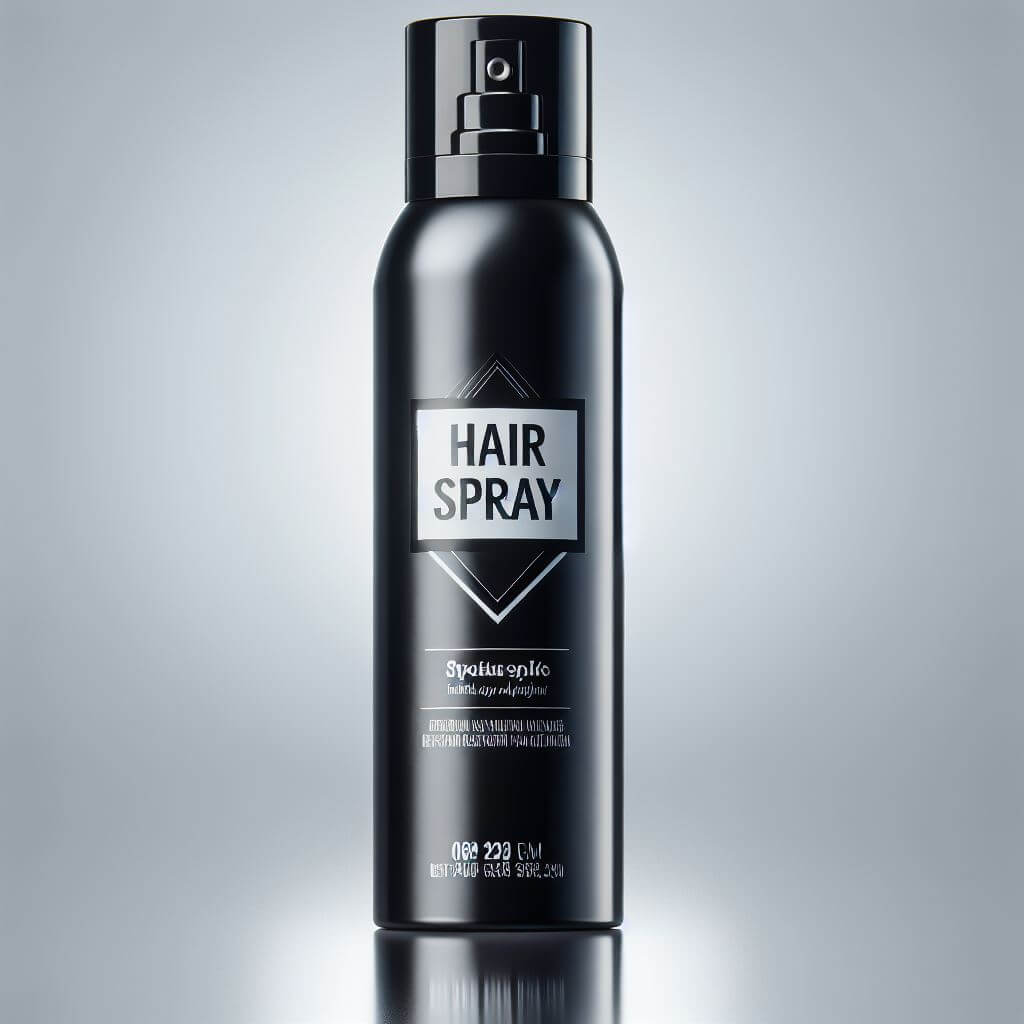
\includegraphics[width=0.5\textwidth,trim={4cm 0 4cm 0},clip]{assets/figures/etat_art/airspray.jpeg}

    \caption{Bombe de laque (IA)}
\end{figure}
Cette solution étant assez sommaire et peu reproductible, elle a été abandonnée au profit de méthodes plus contrôlables.
La durée du "pschit" est sujette à l'erreur humaine, la quantité de liquide projetée
dépend directement de la durée d'appui mais aussi de la pression du gaz de la bombe, cette
dernière diminuant au fil des usages et variant en fonction de la température et de l'altitude,
explique pourquoi cette solution ne fut pas sélectionnée.

% Please add the following required packages to your document preamble:
% \usepackage[table,xcdraw]{xcolor}
% Beamer presentation requires \usepackage{colortbl} instead of \usepackage[table,xcdraw]{xcolor}
\begin{table}[H]
    \centering
    \begin{tabular}{|c|c|lll}
        \cline{1-2}
        Avantages                                 & Inconvénients                                                          &  &  & \\ \cline{1-2}
        \cellcolor[HTML]{67FD9A}Abordable         & \cellcolor[HTML]{FD6864}Durée de "pschit" hasardeuse                   &  &  & \\ \cline{1-2}
        \cellcolor[HTML]{67FD9A}trouvable partout & \cellcolor[HTML]{FD6864}Dépendante de la température et de la pression &  &  & \\ \cline{1-2}
                                                  & \cellcolor[HTML]{FD6864}Très artisanal                                 &  &  & \\ \cline{1-2}
    \end{tabular}
    \caption{Résumé des avantages et inconvénients du spray}
    \label{tab:hair_spray_table}
\end{table}

\newpage
\subsubsection{Aérographe} \label{section_aerographe}
L'aérographe est un pistolet à peinture miniature similaire à un pistolet généralement utilisé pour les traveaux de précision
à peinture utilisé par les carrossiers.
Ces derniers sont généralement alimentés à l'aide d'un compresseur et peuvent projeter plusieurs médiums.

\begin{figure}[H]
    \centering
    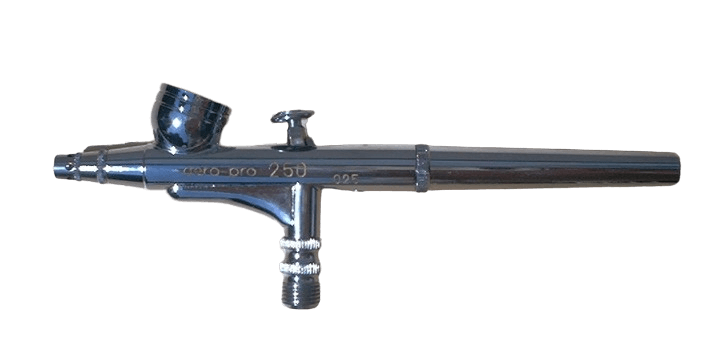
\includegraphics[width=0.8\textwidth]{assets/figures/etat_art/airbrush.png}
    \caption[Aérographe]{Aérographe \cite{airbrush_pics}\footnotemark}
\end{figure}
\footnotetext{\url{http://ingo-karkat.de/textilepainting/About\%20used\%20tools/index.html}}

L'aérographe repose sur l'effet venturi, l'air comprimé entraine le liquide à projeter dans l'embouchure assez fine de l'outil
transformant ce dernier en goutelettes plus ou moins fines en fonction du réglage de l'aiguille de l'outil.

\begin{figure}[H]
    \centering
    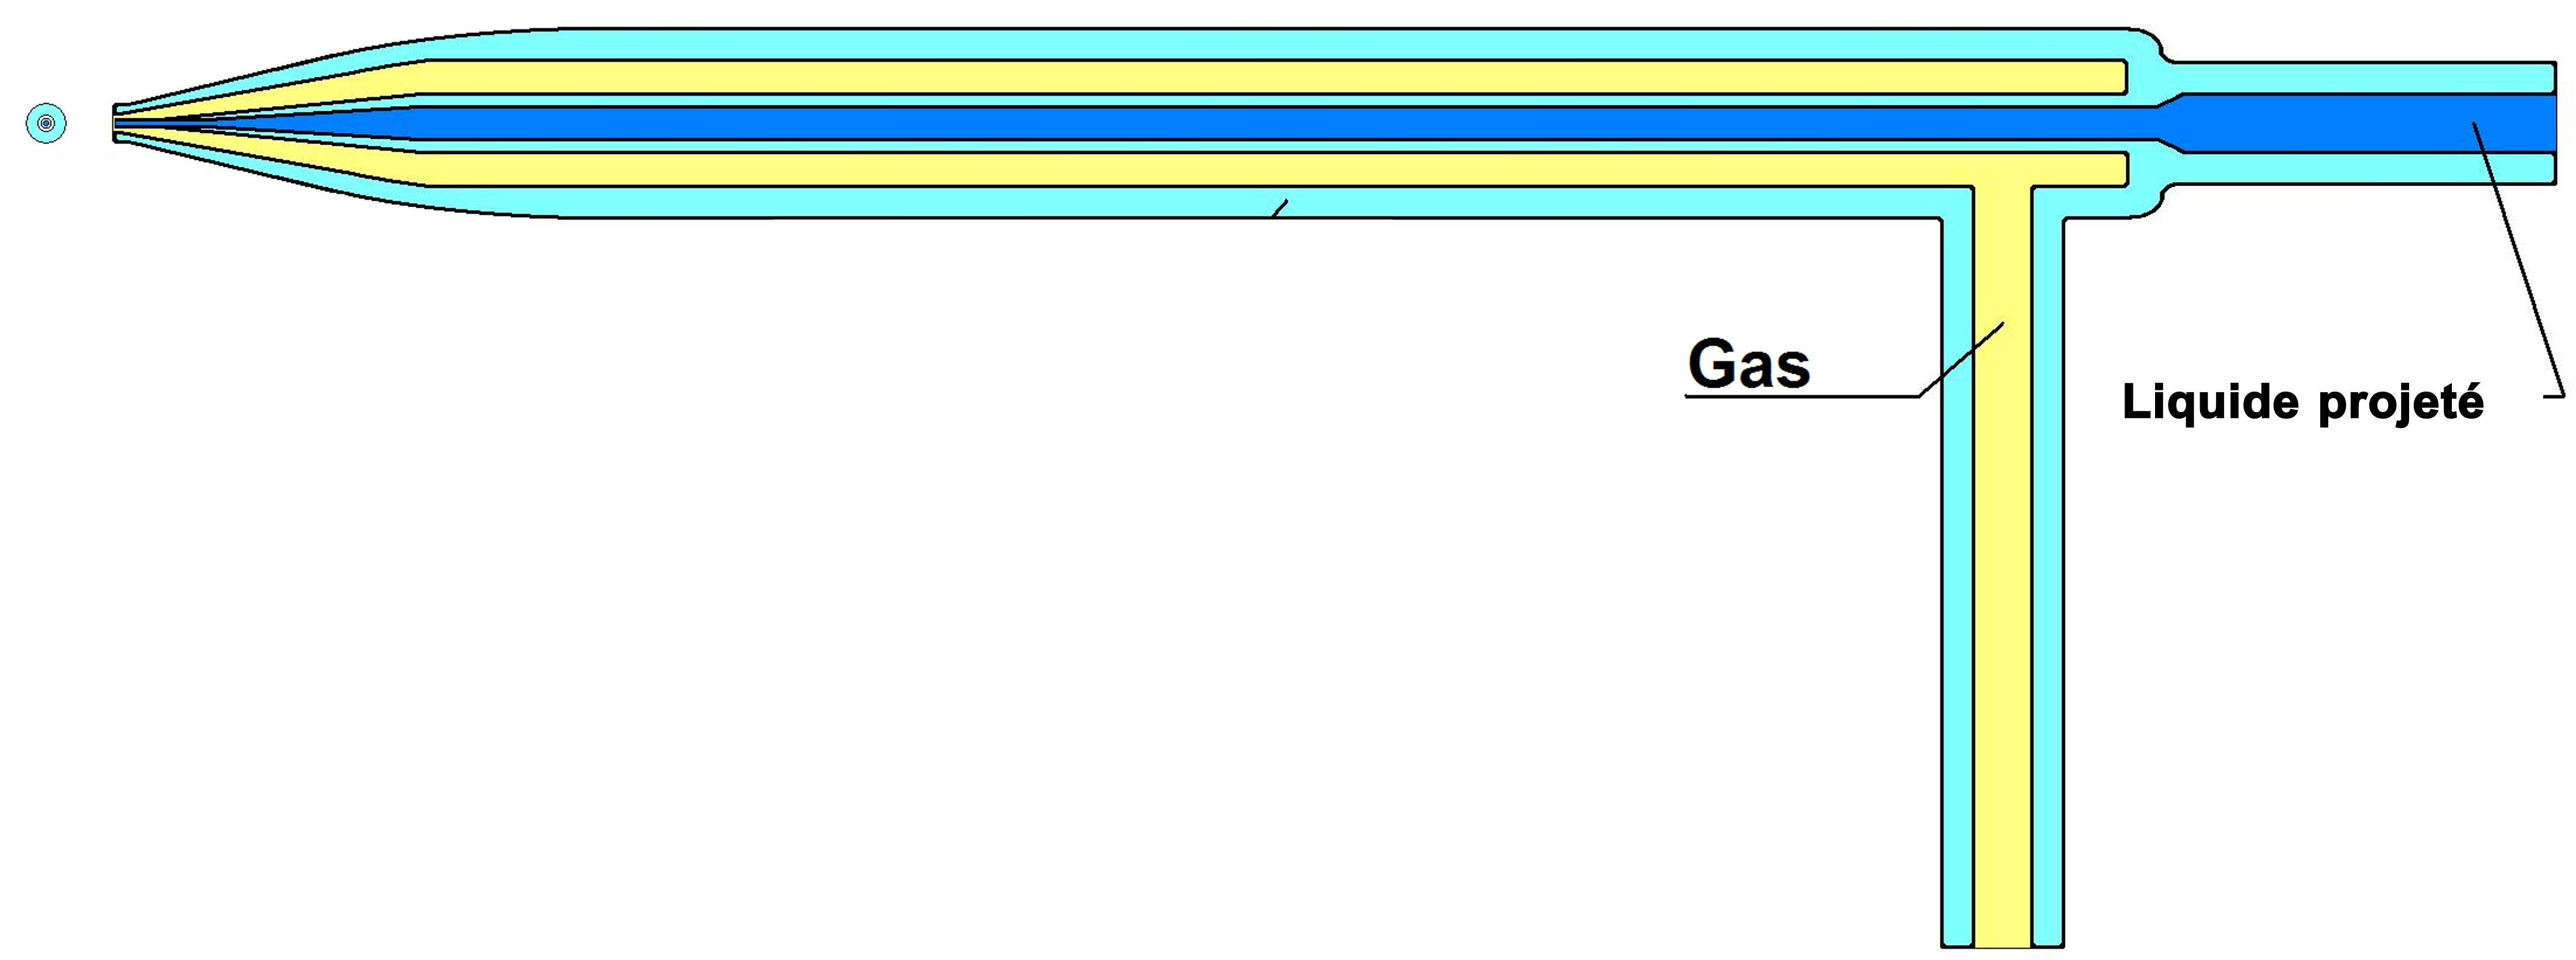
\includegraphics[width=0.6\textwidth]{assets/figures/etat_art/effet_venturi_aerographe.jpg}
    \caption[Effet venturi dans aérographe]{Effet venturi dans aérographe \cite{venturi_airbrush}\footnotemark}
\end{figure}
\footnotetext{\url{https://upload.wikimedia.org/wikipedia/commons/1/1e/Nebulizzatoe\_concentrico.png}}

C'est la solution de projection selectionnée dans la machine actuelle, il a pour avantage, d'être réglable assez finement
et de ne nécessiter qu'un compresseur, le critère de selection principal lors du choix effectué par le concepteur de la machine
était la disponibilité de l'outil de façon rapide en l'empruntant à un tier.

\begin{table}[H]
    \centering
    \begin{tabular}{|c|c|lll}
        \cline{1-2}
        Avantages                                                                                            & Inconvénients                                     &  &  & \\ \cline{1-2}
        \cellcolor[HTML]{67FD9A}Non influencé par l'environnement                                            & \cellcolor[HTML]{FD6864}Montage actuel capricieux &  &  & \\ \cline{1-2}
        \cellcolor[HTML]{67FD9A}Motorisable -\textgreater reproductible                                      & \cellcolor[HTML]{FFFFFF}                          &  &  & \\ \cline{1-2}
        \cellcolor[HTML]{67FD9A}Beaucoup de possibilités de modifier la brumisation                          & \cellcolor[HTML]{FFFFFF}                          &  &  & \\ \cline{1-2}
        \multicolumn{1}{|l|}{\cellcolor[HTML]{67FD9A}Possibilité de contrôler la composition de l'acrylique} & \multicolumn{1}{l|}{}                             &  &  & \\ \cline{1-2}
    \end{tabular}
    \caption{Résumé des avantages et inconvénients de l'aérographe}
    \label{tab:aerographe_table}
\end{table}

\subsubsection{Atomiseurs pneumatiques}
Les atomiseurs pneumatiques reposent sur le même principe de fonctionnement que l'aérographe de la \autoref{section_aerographe}